\documentclass[10pt, letterpaper]{book}
\usepackage[english]{babel} % Explicit language
\usepackage[T1]{fontenc} % Encoding
\usepackage[utf8]{inputenc} % Encoding
\usepackage{lmodern} % Font
\usepackage{graphicx} % To insert figures
\usepackage{hyperref} % Clickable links
\usepackage{amssymb} % math stuffs
\usepackage{amsmath}
\hypersetup{
    colorlinks,
    citecolor=black,
    filecolor=black,
    linkcolor=black,
    urlcolor=black,
    pageanchor=false
}

\usepackage[left=3cm, right=3cm, bottom=4cm, top=4cm]{geometry} % Borders

% \newtheorem{defn}{Definition}
% \newtheorem{coro}{Corollary}
% \newtheorem{conjec}{Conjecture}
% \newtheorem{example}{Example}
% \newtheorem{Lem}{Lemma}
% \newtheorem{fact}{Fact}
% \newtheorem{prop}{{\bf Proposition}}

\renewcommand{\vec}[1]{\mathbf{#1}}


% \newcommand{\ol}[1]{\overline{#1}}
% \newcommand{\mr}[1]{\mathrm{#1}}
% \newcommand{\tx}[1]{\textrm{#1}}
\newcommand{\tr}[1]{{#1}^\top}

% \newcommand{\Om}{\Omega}
% \newcommand{\UU}{\mathcal{U}}
\newcommand{\CC}{\mathcal{C}}
% \newcommand{\TT}{\mathcal{T}}
% \newcommand{\QQ}{\mathcal{Q}}
% \newcommand{\II}{\mathcal{I}}
% \newcommand{\FF}{\mathcal{F}}
% \newcommand{\RR}{\mathbb{R}}
% \newcommand{\XX}{\mathcal{X}}
% \newcommand{\HH}{\mathcal{H}}
% \newcommand{\DD}{\mathcal{D}}
% \newcommand{\BB}{\mathcal{B}}
% \newcommand{\SSS}{\mathcal{S}}
% \newcommand{\NN}{\mathcal{N}}
\newcommand{\LL}{\mathcal{L}}
% \newcommand{\PP}{\mathrm{Pr}}
% \newcommand{\ppi}{\vec \pi}
\newcommand{\pp}{\vec p}
% \newcommand{\qq}{\vec q}
% \newcommand{\dd}{\vec d}
% \newcommand{\cc}{\vec c}
% \newcommand{\CX}{\overline{X}}
% \newcommand{\ax}{\tilde x}
% \newcommand{\kk}{\vec k}
% \newcommand{\va}{\vec a}
% \newcommand{\hx}{\hat{\vec x}}
% \newcommand{\hy}{\widehat{\vec y}}
% \newcommand{\hu}{\widehat{\vec u}}
% \newcommand{\hW}{\widehat{W}}
% \newcommand{\hD}{\widehat{D}}
% \newcommand{\hL}{\widehat{L}}
% \newcommand{\hU}{\hat{U}}
% \newcommand{\hA}{\hat{A}}
% \newcommand{\hY}{\hat{Y}}
% \newcommand{\hV}{\hat{V}}
% \newcommand{\hS}{\hat{\Sigma}}
% \newcommand{\mx}{\overline{\vec x}}
% \newcommand{\hX}{\hat{X}}
% \newcommand{\yy}{\vec y}
\newcommand{\vo}{\vec 1}
% \newcommand{\vz}{\vec 0}
% \newcommand{\ww}{\vec w}
% \newcommand{\zz}{\vec z}
% \newcommand{\bb}{\beta}
% \newcommand{\s}{s}
% \newcommand{\ee}{\vec e}
\newcommand{\uu}{\vec u}
\newcommand{\ff}{\vec f}
% \newcommand{\hh}{\vec h}
% \newcommand{\rr}{\vec r}
\newcommand{\aaa}{\boldsymbol{\alpha}}
% \newcommand{\bbb}{\boldsymbol{\beta}}
\newcommand{\ttt}{\boldsymbol{\theta}}
% \newcommand{\ssim}{\mathrm{sim}}
% \newcommand{\ssum}{\sum\limits}
% \DeclareMathOperator*{\argmax}{arg\,max}
% \DeclareMathOperator*{\argmin}{arg\,min}
% \DeclareMathOperator*{\trace}{tr}
% \DeclareMathOperator*{\diag}{diag}
% \DeclareMathOperator*{\rank}{rank}

% %\def\Rt{\mathbb{R}^{2}}
% %\def\Rn{\mathbb{R}^{n}}
\def\real{{\mathbb R}}
% %\def\natural{{\mathbb N}}
% %\def\C{{\mathbf \chi}}
% %\newcommand{\vecprod}[2]{\left\langle#1,#2\right\rangle}

% \def\httilde{\mbox{\tt\raisebox{-.5ex}{\symbol{126}}}}

% \newcommand{\vnu}{\boldsymbol \nu}
% \newcommand{\lu}{\tr\uu L\uu}
% \newcommand{\lz}{\tr\zz L\zz}
% \newcommand{\vF}{\vec F}
% \newcommand{\vv}{\vec v}

\begin{document}
    \begin{titlepage}
    \centering
    
\includegraphics[width=0.3\textwidth]{figure/ets_logo}\par\vspace{1cm}
    {\scshape\LARGE ÉTS Montréal\par}
    \vspace{1cm}
    {\scshape\Large Class/goal\par}
    \vspace{1.5cm}
    {\huge\bfseries Main title\par}
    {\Large\itshape Sub title\par}
    \vspace{2cm}
    {\Large Hoel \textsc{Kervadec}\par}
    \vfill
    supervised by\par
    Dr.~John \textsc{Doe}

    \vfill

% Bottom of the page
    {\large \today\par}
\end{titlepage}

    \frontmatter
    \chapter*{\centering Abstract}
        Ce n'est qu'en essayant continuellement que l'on finit par réussir.
        En d'autres termes: plus ça rate et plus on a de chances que ça marche.
    \setcounter{tocdepth}{2}
    \tableofcontents

    \addcontentsline{toc}{chapter}{List of Figures}
    \listoffigures

    \addcontentsline{toc}{chapter}{List of Tables}
    \listoftables

    \setlength{\parskip}{5pt}

    \chapter{List of symbols}
    \begin{table}[h]
        \centering
        \begin{tabular}{|c|l|}
            \hline
                $I$ & Input image \\
            \hline
                $N$ & Number of pixels of $I$ \\
            \hline
                $\vec x = [x_1,x_2,...,x_N]$ & Set of random variables, written as a vector\\
            \hline
                $\{1,...,L\}$ & Different labels \\
            \hline
        \end{tabular}
    \end{table}

    \mainmatter
    \chapter{Introduction}
    This small template is aimed at making my life easier in the future.

    I will add with time a list of useful packages and what they do, to avoid too much bloat in new projects.

    \chapter{Content}
    \section{Figures}
        Below a few examples of figures, especially in a two columns environment.
        First, remember that Figure \ref{fig:intro:shadoko} is always here to help.

        \begin{figure}[h]
            \centering
            
\includegraphics[width=0.4\textwidth]{figure/intro/shadoko}
            \label{fig:intro:shadoko}
            \caption{Professor Shadoko explains something.\cite{denis2012de}}
        \end{figure}

        \subsection{}
            For figures that takes the whole page, see the code of Figure \ref{fig:intro:widsom}.
            \begin{figure*}[h]
                \centering
                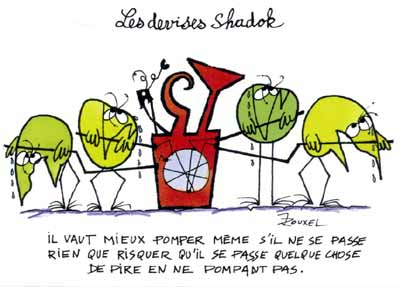
\includegraphics[width=1\textwidth]{figure/intro/wisdom}
                \label{fig:intro:widsom}
                \caption{Some French common wisdom.}
            \end{figure*}

    \section{Tables}
        Tables are great to display too much number, as in Table \ref{tab:supertable}

        \begin{table}[h]
            \centering
            \begin{tabular}{|r|r|}
                \hline
                X & X \\
                \hline
                .5 & .5 \\
                \hline
                1 & 1 \\
                \hline
            \end{tabular}
            \label{tab:supertable}
            \caption{X value over X}
        \end{table}

    \section{Maths}
        There is different ways to include maths, as $f(x) = \sum_i x_i$, \[ f(x) = \sum_i x_i, \] or even with a proper equation (Equation \eqref{eq:proper}):
        \begin{equation}
            \label{eq:proper}
            f(x) = \sum_i x_i
        \end{equation}

    \section{Conclusion}
    This was really useful.

    \appendix
    \chapter{Citations très interessantes}
    \section{Dune}
        « Je ne connaîtrai pas la peur, car la peur tue l'esprit. La peur est la petite mort qui conduit à l'oblitération totale. J'affronterai ma peur. Je lui permettrai de passer sur moi, au travers de moi. Et lorsqu'elle sera passée, je tournerai mon œil intérieur sur son chemin. Et là où elle sera passée, il n'y aura plus rien. Rien que moi. »

    \bibliographystyle{plain}
    \bibliography{input/biblio}
\end{document}
